\documentclass[a4paper,titlepage]{article}
\usepackage[utf8]{inputenc}
\usepackage{fullpage}
\usepackage{indentfirst}
\usepackage[per-mode=symbol]{siunitx}
\usepackage{listings}
\usepackage{graphicx}
\usepackage{color}
\usepackage{amsmath}
\usepackage{array}
\usepackage[hidelinks]{hyperref}
\usepackage[format=plain,font=it]{caption}
\usepackage{subcaption}
\usepackage{standalone}
\usepackage[nottoc]{tocbibind}
\usepackage[noabbrev,capitalize,nameinlink]{cleveref}
\usepackage{listings}
\usepackage{xspace}
\usepackage{tikz}
\usepackage{circuitikz}
\usepackage{titlesec}
\usepackage[cache=false]{minted}
\usepackage{booktabs}
\usepackage{csvsimple}
\newcommand{\MATLAB}{\textsc{Matlab}\xspace}
\usepackage{siunitx}
\usepackage[super]{nth}
\usepackage[titletoc]{appendix}

% Custom commands
\newcommand\numberthis{\addtocounter{equation}{1}\tag{\theequation}}
\newcommand{\code}[1]{\texttt{#1}}
\newcolumntype{P}[1]{>{\centering\arraybackslash}p{#1}}

\setminted{linenos,breaklines,fontsize=auto}

%\titleformat*{\section}{\normalsize\bfseries}
%\titleformat*{\subsection}{\small\bfseries}
\renewcommand{\thesubsection}{\thesection.\alph{subsection}}
\providecommand*{\listingautorefname}{Listing}
\newcommand*{\Appendixautorefname}{Appendix}


\begin{document}
	\sloppy	
	
	\begin{center}
		{\LARGE \bf ECSE 597: Circuit Simulations and Modeling}\\
		{\large Assignment 3, \quad \today}\\
		{\large Wenjie Wei, 260685967}
	\end{center}

	
	\section{Chebychev Filter}		
		\MATLAB code listings will be presented at the end of the document. Figures \ref{chebychev_mag} and \ref{chebychev_angle} below show the magnitude and angular response of the Chebychev filter. 
		
		\begin{figure}[H]
			\centering
			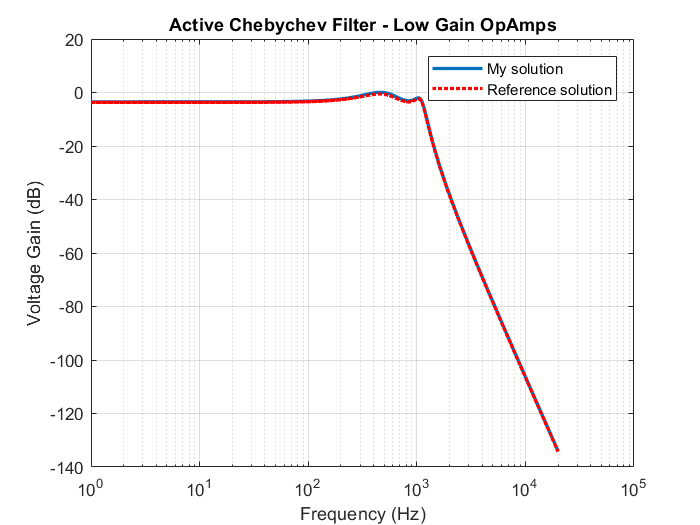
\includegraphics[width=0.7\linewidth]{../../src/a3/plots/chebychev_gain}
			\caption{Magnitude Response of the Chebychev Filter}
			\label{chebychev_mag}
		\end{figure}
		\begin{figure}[H]
			\centering
			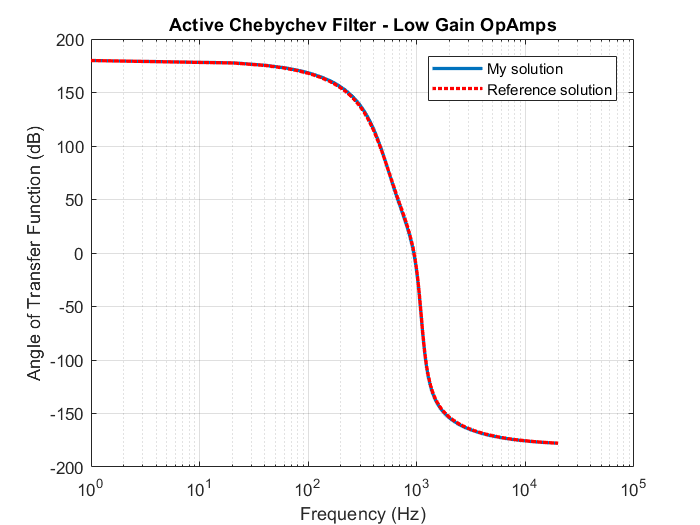
\includegraphics[width=0.7\linewidth]{../../src/a3/plots/chebychev_angle}
			\caption{Angular Response of the Chebychev Filter}
			\label{chebychev_angle}
		\end{figure}
	
	\newpage
	\section{Large Gain Chebychev Filter}
	
		Figures \ref{chebychev_large_mag} and \ref{chebychev_large_angle} below show the magnitude and angular response of the large gain Chebychev filter. 
		
		\begin{figure}[H]
			\centering
			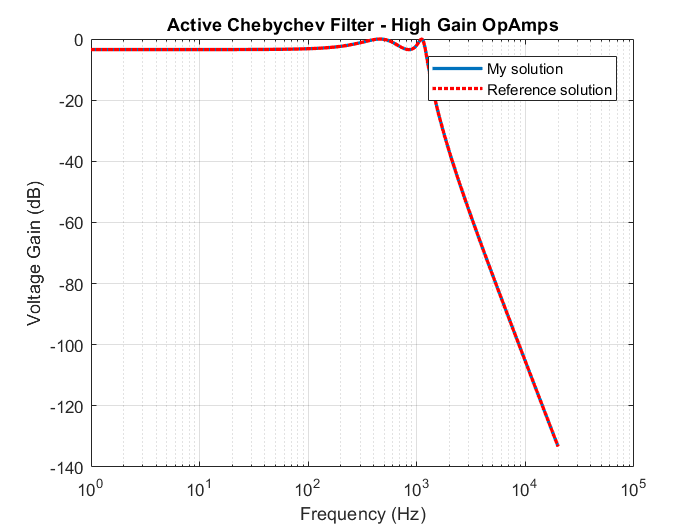
\includegraphics[width=0.7\linewidth]{../../src/a3/plots/chebychev_large_gain}
			\caption{Magnitude Response of the Large Gain Chebychev Filter}
			\label{chebychev_large_mag}
		\end{figure}
		\begin{figure}[H]
			\centering
			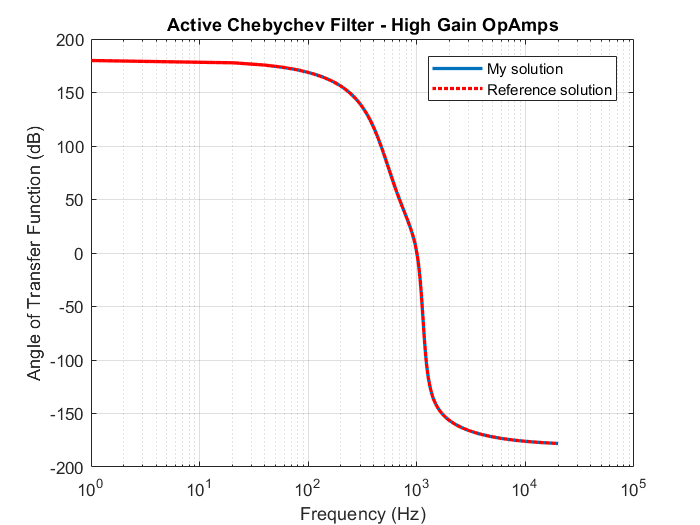
\includegraphics[width=0.7\linewidth]{../../src/a3/plots/chebychev_large_angle}
			\caption{Angular Response of the Large Gain Chebychev Filter}
			\label{chebychev_large_angle}
		\end{figure}
	
	\newpage
	\section{Circuit 4 Test Bench}
		Figures \ref{cir4_mag} and \ref{cir4_angle} below show the magnitude and angular response of the Circuit 4 Test Bench. 
		
		\begin{figure}[H]
			\centering
			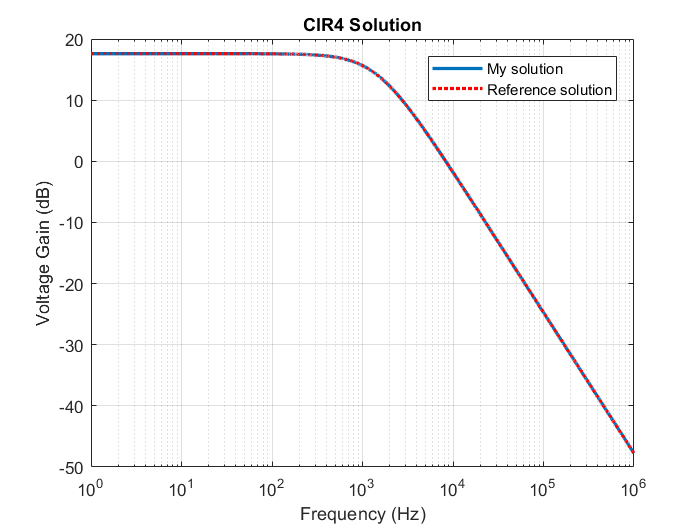
\includegraphics[width=0.7\linewidth]{../../src/a3/plots/cir4_gain}
			\caption{Magnitude Response of the Circuit 4 Test Bench}
			\label{cir4_mag}
		\end{figure}
		\begin{figure}[H]
			\centering
			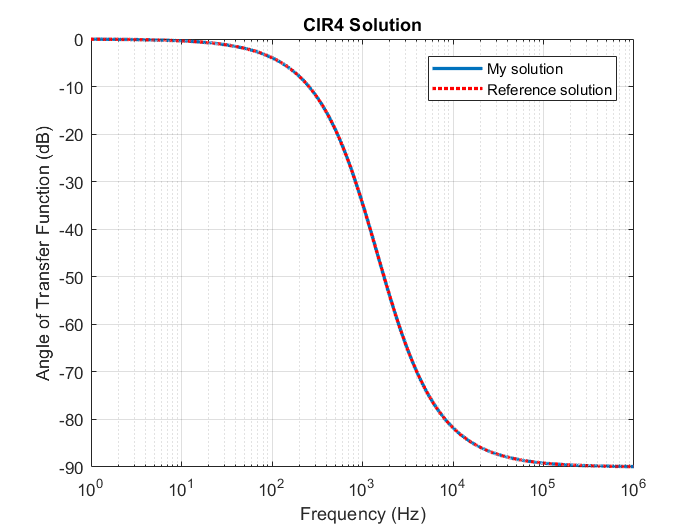
\includegraphics[width=0.7\linewidth]{../../src/a3/plots/cir4_angle}
			\caption{Angular Response of the Circuit 4 Test Bench}
			\label{cir4_angle}
		\end{figure}
		
		\newpage
		\section{LC Filter 1 Test Bench}
		Figures \ref{lc1_mag} and \ref{lc1_angle} below show the magnitude and angular response of the LC Filter 1 Test Bench. 
		
		\begin{figure}[H]
			\centering
			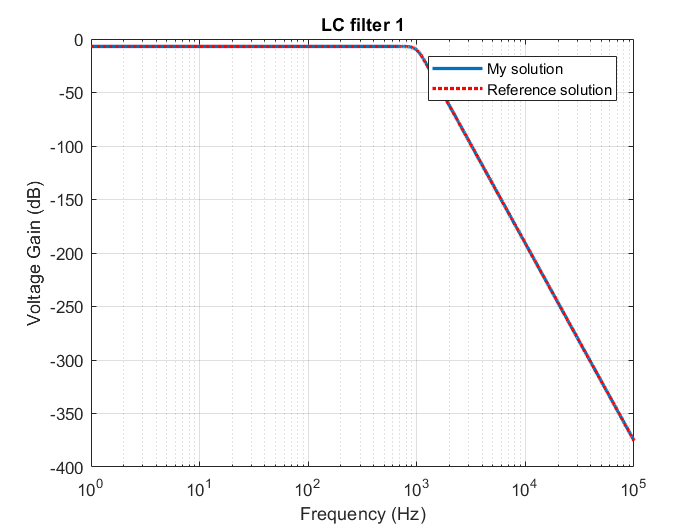
\includegraphics[width=0.7\linewidth]{../../src/a3/plots/LCFilter1_gain}
			\caption{Magnitude Response of the LC Filter 1 Test Bench}
			\label{lc1_mag}
		\end{figure}
		\begin{figure}[H]
			\centering
			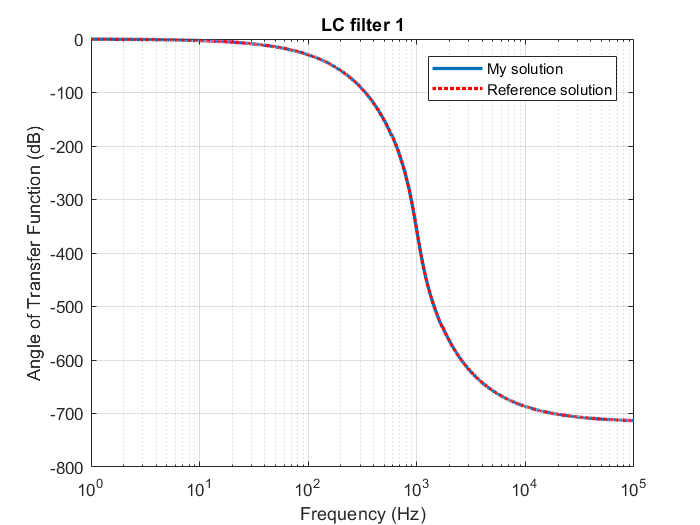
\includegraphics[width=0.7\linewidth]{../../src/a3/plots/LCFilter1_angle}
			\caption{Angular Response of the LC Filter 1 Test Bench}
			\label{lc1_angle}
		\end{figure}
		
		\newpage
		\section{LC Filter 2 Test Bench}
		Figures \ref{lc2_mag} and \ref{lc2_angle} below show the magnitude and angular response of the LC Filter 2 Test Bench. 
		
		\begin{figure}[H]
			\centering
			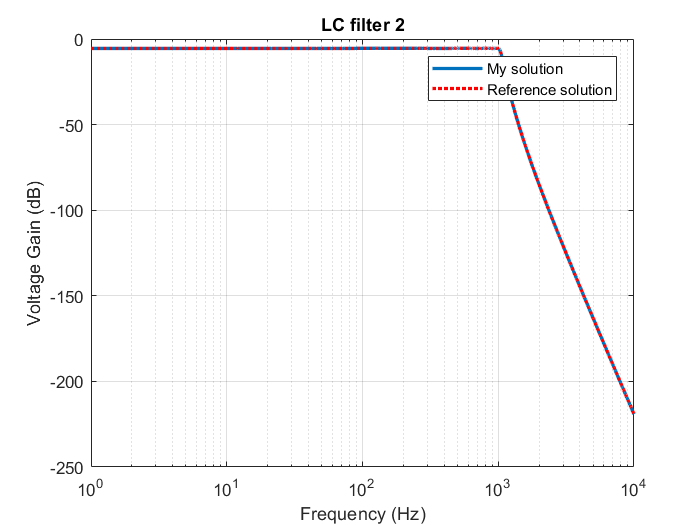
\includegraphics[width=0.7\linewidth]{../../src/a3/plots/LCFilter2_gain}
			\caption{Magnitude Response of the LC Filter 2 Test Bench}
			\label{lc2_mag}
		\end{figure}
		\begin{figure}[H]
			\centering
			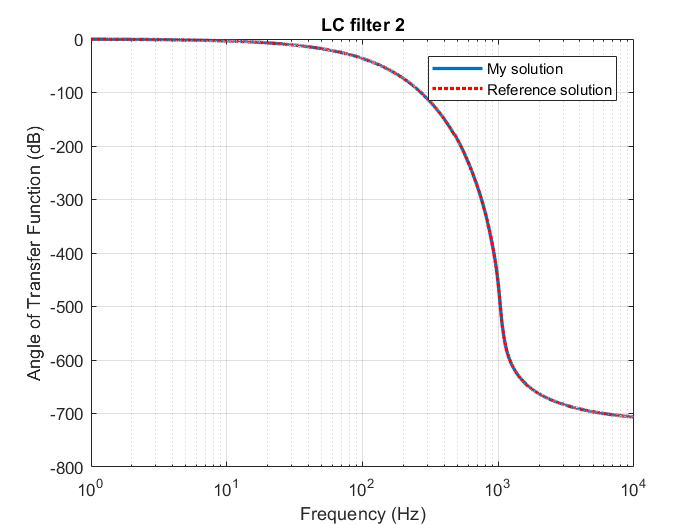
\includegraphics[width=0.7\linewidth]{../../src/a3/plots/LCFilter2_angle}
			\caption{Angular Response of the LC Filter 2 Test Bench}
			\label{lc2_angle}
		\end{figure}
	
		\newpage
		\section{LC Filter 3 Test Bench}
		Figures \ref{lc23_mag} and \ref{lc3_angle} below show the magnitude and angular response of the LC Filter 3 Test Bench. 
		
		\begin{figure}[H]
			\centering
			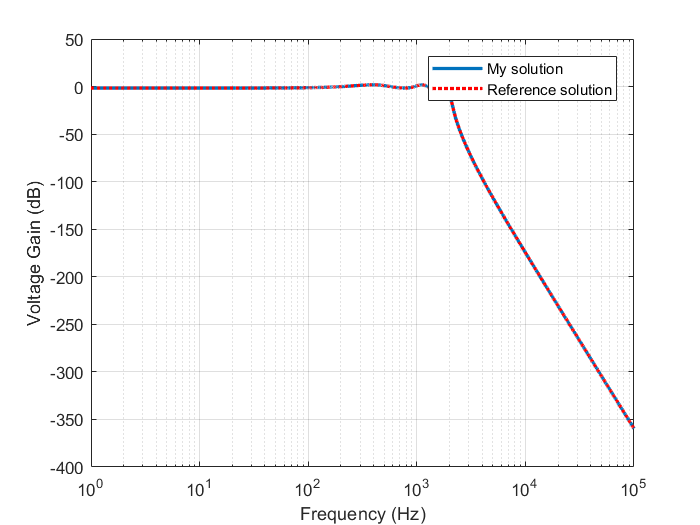
\includegraphics[width=0.7\linewidth]{../../src/a3/plots/LCFilter3_gain}
			\caption{Magnitude Response of the LC Filter 3 Test Bench}
			\label{lc3_mag}
		\end{figure}
		\begin{figure}[H]
			\centering
			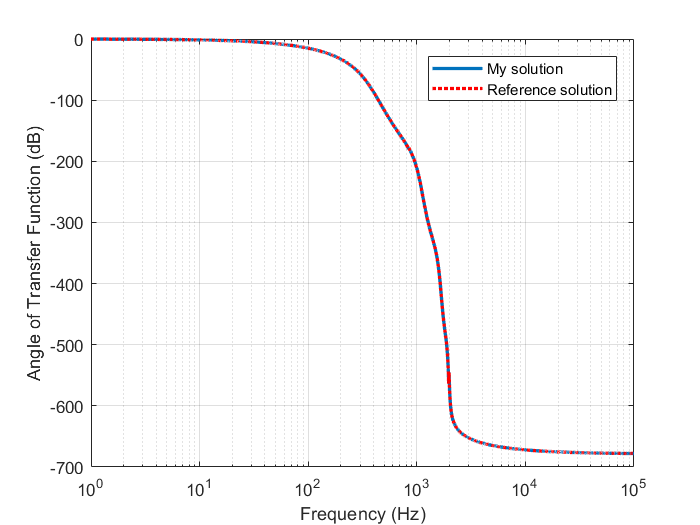
\includegraphics[width=0.7\linewidth]{../../src/a3/plots/LCFilter3_angle}
			\caption{Angular Response of the LC Filter 3 Test Bench}
			\label{lc3_angle}
		\end{figure}
	
	\newpage
	\begin{appendices}
		
		\section{Code Listings} \label{appendix:code}
		
		\setminted{linenos,breaklines,fontsize=\footnotesize}
		
		\begin{center}
			\captionof{listing}{MATLAB Function to Compute the Frequency Response (\texttt{fsolve.m}).}
			\inputminted{matlab}{../../src/a3/fsolve.m}
			\label{fsolve}
		\end{center}
		
		\begin{center}
			\captionof{listing}{MATLAB Function to Generate Inductance Matrices (\texttt{ind.m}).}
			\inputminted{matlab}{../../src/a3/ind.m}
			\label{ind}
		\end{center}
	
		\begin{center}
			\captionof{listing}{MATLAB Function to Generate VCCS Matrices (\texttt{vccs.m}).}
			\inputminted{matlab}{../../src/a3/vccs.m}
			\label{vccs}
		\end{center}
		\begin{center}
			\captionof{listing}{MATLAB Function to Generate VCVS Matrices (\texttt{vccs.m}).}
			\inputminted{matlab}{../../src/a3/vcvs.m}
			\label{vcvs}
		\end{center}
	\end{appendices}
\end{document}